\chapter{Configuration interaction}
    The most natural approach to take in quantum mechanics when creating a wave
    function is to create a linear combination of all possible states contained
    in the space one is exploring.
    Configuration interaction is a procedure which creates a many-body wave
    function from a linear combination of all possible Slater determinants in
    the basis of spin-orbitals that is given, viz.
    \begin{align}
        \ket{\Psi}
        &= C\ketslat
        + C^a_i\ketslate{a}{i}
        + \frac{1}{4}C^{ab}_{ij}\ketslate{ab}{ij}
        + \dots,
        \label{eq:ci_wavefunction}
    \end{align}
    where we have divided by a factor $4$ in the double sum to avoid over
    counting as both the coefficients and the excited determinants are
    antisymmetric.
    This leads to a method which is highly understandable for everyone with a
    background in quantum mechanics.
    Not to mention that it is a method that is exact within the given space,
    variational, stable, single- and multi-reference, and yields the full
    spectrum, i.e., all excited states and energies, for the many-body
    Hamiltonian.
    The method is extensible to the time-domain in a natural way and exhibits
    the same properties as mentioned above.

    There is however a significant catch to the configuration interaction
    method, and that is its computational scaling.
    The number of Slater determinants $N_{s}$ for a given basis of $L$
    spin-orbitals with $N$ occupied particles will grow as \cite{kvaal2017notes}
    \begin{align}
        N_{s} = \binom{L}{N}.
    \end{align}
    This is such a significant roadblock that the method very quickly becomes
    completely infeasible for systems of interest.
    Significant attempts at lowering the cost of configuration interaction has
    been explored, but the factorial scaling quickly rears its ugly head at a
    certain point unless drastic measures are done which inevitably destroys
    some of the pleasant properties of the method.
    % TODO: Cite some of these attempts

    A word on notation, we will in the following refrain from using explicit
    excitation indices $a, b, \dots$ and $i, j, \dots$ when labelling excited
    Slater determinants, but rather label the
    coefficients and the Slater determinants by capital letter $I, J, K,
    \dots$.
    That is, we can write \autoref{eq:ci_wavefunction} on the short form
    \begin{align}
        \ket{\Psi}
        &= C_{I}\ket{\Phi_I}.
    \end{align}
    The capital indices will then run over the total number of Slater
    determinants $N_s$ in the full Slater determinant basis.
    This number will depend on the truncation level of the configuration
    interaction wave function.

    \section{Time-independent configuration interaction}
        We start with the time-independent Schrödinger equation
        \begin{align}
            \hamil\ket{\Psi_J} = E_J\ket{\Psi_J},
            \label{eq:ci_tise}
        \end{align}
        where $(E_J, \ket{\Psi_J})$ is an eigenpair for $\hat{H}$.
        Expanding the CI wavefunction in a Slater determinant basis.
        \begin{align}
            \ket{\Psi_J} = C_{KJ}\ket{\Phi_K},
            \label{eq:expanded_ci_wavefunction}
        \end{align}
        where $C_{KJ}$ are the amplitudes for a certain excitation $K$ for a
        specific energy level $J$.
        Inserting \autoref{eq:expanded_ci_wavefunction} into
        \autoref{eq:ci_tise} and left projecting on a state $\ket{\Phi_I}$ we
        get
        \begin{align}
            \bra{\Phi_I}\hat{H}\ket{\Phi_K}C_{KJ}
            = E_J\braket{\Phi_I}{\Phi_K}C_{KJ}.
        \end{align}
        We now define the Hamiltonian matrix $H_{IK} =
        \bra{\Phi_I}\hat{H}\ket{\Phi_K}$ and the overlap matrix $S_{IK} =
        \braket{\Phi_I}{\Phi_K}$.
        We can thus formulate the generalized eigenvalue equation
        \begin{gather}
            H_{IK}C_{KJ} = E_J S_{IK}C_{KJ}
            \\
            \implies
            HC = ESC,
        \end{gather}
        where $S_{IK} = 1 \iff \braket{\Phi_I}{\Phi_K} = \delta_{IK}$.
        We will in this text only care about systems where the Slater
        determinants are orthonormal.
        Thus the eigenvalue equation we will solve will be
        \begin{align}
            HC = EC,
        \end{align}
        which means our job is to construct $H_{IJ}$ and diagonalize the
        matrix \cite{karwowski}.
        The elements $H_{IJ}$ are computed by
        \begin{align}
            \bra{\Phi_I}\hat{H}\ket{\Phi_J}
            &= h^{p}_{q}
            \bra{\Phi_I}\ccr{p}\can{q}\ket{\Phi_J}
            + \frac{1}{4} u^{pq}_{rs}
            \bra{\Phi_I}\ccr{p}\ccr{q}\can{s}\can{r}\ket{\Phi_J}.
        \end{align}
        Having constructed the one- and two-body elements $h^{p}_{q}$ and
        $u^{pq}_{rs}$ what remains is for us to evaluate the integrals
        $\bra{\Phi_I}\ccr{p}\can{q}\ket{\Phi_J}$ and
        $\bra{\Phi_I}\ccr{p}\ccr{q}\can{s}\can{r}\ket{\Phi_J}$.
        We are then able to construct the configuration interaction matrix
        \begin{align}
            \hamilmat
            &=
            \begin{pmatrix}
                \bra{\Phi_0}\hamil\ket{\Phi_0} &
                \bra{\Phi_0}\hamil\ket{\Phi_1} &
                \dots &
                \bra{\Phi_0}\hamil\ket{\Phi_{N_s}} \\
                \bra{\Phi_1}\hamil\ket{\Phi_0} &
                \bra{\Phi_1}\hamil\ket{\Phi_1} &
                \dots &
                \bra{\Phi_1}\hamil\ket{\Phi_{N_s}} \\
                \vdots & \vdots & \ddots & \vdots \\
                \bra{\Phi_{N_s}}\hamil\ket{\Phi_0} &
                \bra{\Phi_{N_s}}\hamil\ket{\Phi_1} &
                \dots &
                \bra{\Phi_{N_s}}\hamil\ket{\Phi_{N_s}}
            \end{pmatrix}.
        \end{align}
        It is common to see this matrix in block form where we collect
        the different excitation levels in separate blocks.
        For the singles and doubles excitations we get the block matrix
        \begin{align}
            \hamilmat_{\text{CISD}}
            &=
            \begin{pmatrix}
                \bra{\Phi}\hamil\ket{\Phi} &
                \bra{\Phi}\hamil\ket{\Phi^{a}_{i}} &
                \bra{\Phi}\hamil\ket{\Phi^{ab}_{ij}} \\
                \bra{\Phi^{c}_{k}}\hamil\ket{\Phi} &
                \bra{\Phi^{c}_{k}}\hamil\ket{\Phi^{a}_{i}} &
                \bra{\Phi^{c}_{k}}\hamil\ket{\Phi^{ab}_{ij}} \\
                \bra{\Phi^{cd}_{kl}}\hamil\ket{\Phi} &
                \bra{\Phi^{cd}_{kl}}\hamil\ket{\Phi^{a}_{i}} &
                \bra{\Phi^{cd}_{kl}}\hamil\ket{\Phi^{ab}_{ij}} \\
            \end{pmatrix}.
        \end{align}

        \subsection{Truncated configuration interaction}
            \label{sub:truncated-configuration-interaction}
            % TODO: Demonstrate truncated configuration interaction and discuss
            % its disadvantages such as lack of size extensivity and size
            % consistency.
            As discussed at the top of this chapter, the full configuration
            interaction method quickly encounters exponential scaling and
            becomes intractable.
            A common technique utilized to lower the cost of the method is to
            only include Slater determinants based on their excitation.
            For example, by only including the doubly excited Slater
            determinants, we can construct the configuration interaction doubles
            (CID) wave function by
            \begin{align}
                \ket{\Psi} = C\ketslat
                + \frac{1}{4} C^{ab}_{ij} \ket{\slat^{ab}_{ij}},
            \end{align}
            which reduces the number of Slater determinants to
            \begin{align}
                N_s = 1 + \left\lfloor\frac{N(N - 1)(L - N)(L - N -
                1)}{4}\right\rfloor,
            \end{align}
            where the division is floored to the nearest integer.
            Defining $M = L - N$ as the number of virtual spin-orbitals, the
            scaling of the number of Slater determinants in the configuration
            interaction doubles method is given by
            \begin{align}
                N_s = \mathcal{O}(N^2 M^2),
            \end{align}
            which is significant deacrease in computational complexity.
            However, due to the truncation of the wave function not only do we
            deacrease the quality of the method in terms of closeness to the
            exact solution given by full configuration interaction, we also lose
            many of the other properties.
            % TODO: List and explain the properties lost, e.g., multi-reference,
            % size-exensivity, size consistency.

            \subsubsection{The singles approximation on a small basis}
                As an example of <size extensivity/size consistency> we demonstrate
                the troubles arising when we restrict ourselves to a system of two
                particles and four basis functions.
                Our basis thus consists of the spin-orbitals $\brac{\ket{\phi_p},
                }_{p = 1}^{4}$, with the reference Slater determinant
                \begin{align}
                    \ket{\Phi}
                    &= \frac{1}{\sqrt{2}}\brac{
                        \ket{\phi_1\phi_2}
                        - \ket{\phi_2\phi_1}
                    }.
                    % TODO: It might not be necessary to show what the determinant
                    % looks like.
                \end{align}
                Using truncated configuration interaction with singles excitations
                only, we get the many-body wave function
                \begin{align}
                    \ket{\Psi}
                    &= C\ket{\Phi}
                    + C^{a}_{i}\ket{\Phi^{a}_{i}}
                    = C\ket{\Phi}
                    + C^{3}_{1}\ket{\Phi^{3}_{1}}
                    + C^{4}_{1}\ket{\Phi^{4}_{1}}
                    + C^{3}_{2}\ket{\Phi^{3}_{2}}
                    + C^{4}_{2}\ket{\Phi^{4}_{2}}.
                    \label{eq:cis_wave_function}
                \end{align}
                Graphically we can represent the full space of the Slater determinants
                by \autoref{fig:tiny-slater-basis}.
                Comparing with \autoref{eq:cis_wave_function} we see that the only
                determinant missing in the truncated wave function is the doubly
                excited determinant $\ket{\Phi^{34}_{12}}$.
                Stated a little differently, truncated configuration interaction is
                not able to exploit the full space of Slater determinants.
                The method also fails in ``removing all trace`` of the reference
                state.
                This means that truncated configuration interaction will not be able
                to fully excite the reference state.
                Note that the example shown in \autoref{eq:cis_wave_function} and
                \autoref{fig:tiny-slater-basis} extends for more particles and
                higher truncation levels for configuration interaction.
                For example for a system with four particles and truncated
                configuration interaction with singles and doubles excitations this
                same behaviour is exhibited.
                % TODO: Explain how this problem becomes worse for more basis
                % functions.
                % TODO: Explain how coupled cluster fixes this problem in the
                % chapter on coupled cluster.
                % TODO: Explain size consistency and size extensivity. See Crawford
                % & Schaefer pages 42 and 95.
                \begin{figure}
                    \begin{center}
                        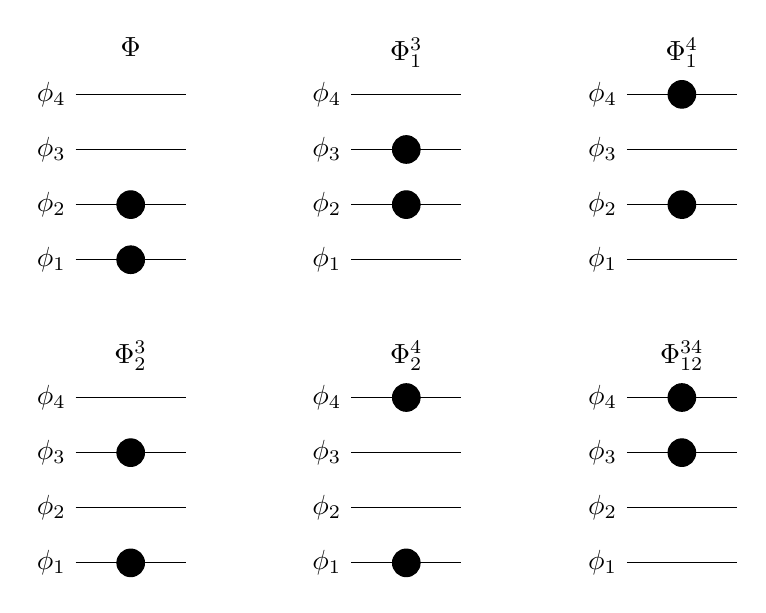
\begin{tikzpicture}[scale=0.7]
                            % State 1
                            \begin{scope}
                                \foreach \i in {1,...,4} {
                                    \draw (-1, \i - 1) node[anchor=east]
                                    {$\ket{\phi_{\i}}$} -- (1, \i - 1);
                                }
                                \filldraw (0,4.2) node[anchor=north]
                                    {$\ket{\Phi}$};
                                \filldraw (0, 0) circle (0.25cm);
                                \filldraw (0, 1) circle (0.25cm);
                            \end{scope}

                            % State 2
                            \begin{scope}[xshift=5cm]
                                \foreach \i in {1,...,4} {
                                    \draw (-1, \i - 1) node[anchor=east]
                                    {$\ket{\phi_{\i}}$} -- (1, \i - 1);
                                }
                                \filldraw (0,4.2) node[anchor=north]
                                    {$\ket{\Phi^{3}_{1}}$};
                                \filldraw (0, 2) circle (0.25cm);
                                \filldraw (0, 1) circle (0.25cm);
                            \end{scope}

                            % State 3
                            \begin{scope}[xshift=10cm]
                                \foreach \i in {1,...,4} {
                                    \draw (-1, \i - 1) node[anchor=east]
                                    {$\ket{\phi_{\i}}$} -- (1, \i - 1);
                                }
                                \filldraw (0,4.2) node[anchor=north]
                                    {$\ket{\Phi^{4}_{1}}$};
                                \filldraw (0, 3) circle (0.25cm);
                                \filldraw (0, 1) circle (0.25cm);
                            \end{scope}

                            % State 4
                            \begin{scope}[yshift=-5.5cm]
                                \foreach \i in {1,...,4} {
                                    \draw (-1, \i - 1) node[anchor=east]
                                    {$\ket{\phi_{\i}}$} -- (1, \i - 1);
                                }
                                \filldraw (0,4.2) node[anchor=north]
                                    {$\ket{\Phi^{3}_{2}}$};
                                \filldraw (0, 0) circle (0.25cm);
                                \filldraw (0, 2) circle (0.25cm);
                            \end{scope}

                            % State 5
                            \begin{scope}[yshift=-5.5cm, xshift=5cm]
                                \foreach \i in {1,...,4} {
                                    \draw (-1, \i - 1) node[anchor=east]
                                    {$\ket{\phi_{\i}}$} -- (1, \i - 1);
                                }
                                \filldraw (0,4.2) node[anchor=north]
                                    {$\ket{\Phi^{4}_{2}}$};
                                \filldraw (0, 0) circle (0.25cm);
                                \filldraw (0, 3) circle (0.25cm);
                            \end{scope}

                            % State 6
                            \begin{scope}[yshift=-5.5cm, xshift=10cm]
                                \foreach \i in {1,...,4} {
                                    \draw (-1, \i - 1) node[anchor=east]
                                    {$\ket{\phi_{\i}}$} -- (1, \i - 1);
                                }
                                \filldraw (0,4.2) node[anchor=north]
                                    {$\ket{\Phi^{34}_{12}}$};
                                \filldraw (0, 3) circle (0.25cm);
                                \filldraw (0, 2) circle (0.25cm);
                            \end{scope}
                        \end{tikzpicture}
                    \end{center}
                    \caption{In this figure we can see the six possible Slater
                    determinants, i.e., all the basis Slater determinants, made from
                    the four basis functions $\brac{\ket{\phi_1}, \ket{\phi_2},
                    \ket{\phi_3}, \ket{\phi_4}}$ with two particles.}
                    \label{fig:tiny-slater-basis}
                \end{figure}

        \subsection{Constructing the Slater determinants}
            % TODO: Explain how to construct bit strings representing
            % determinants.
            % TODO: Discuss Fock space representation of determinants.
            % TODO: Discuss sign of determinants.

        \subsection{Evaluating the matrix elements}
            As the one- and two-body elements $\oneten^{p}_{q}$ and
            $\twoten^{pq}_{rs}$ are known in advance, our task is to evaluate
            the overlap between Slater determinants acted upon by creation and
            annihilation operators.

        \subsection{The Slater-Condon rules}
            When evaluating the matrix elements of the Hamiltonian with at most
            two-body elements between two Slater determinants, we will quickly
            notice that many of the elements are zero.
            The Slater-Condon rules describes which elements are non-zero therby
            greatly reducing the number of matrix elements that need to be
            computed.

        \subsection{One-body density matrix}
            For a given eigenstate $\ket{\Psi_I}$ of the many-body Hamiltonian
            shown in \autoref{eq:ci_tise} we can compute the one-body density
            matrix ${\rho_I}^{q}_{p}$ by
            \begin{align}
                {\rho_I}^{q}_{p}
                &= \bra{\Psi_I}\ccr{p}\can{q}\ket{\Psi_I}
                = C_{JI}^{*}C_{KI}\bra{\Phi_J}\ccr{p}\can{q}\ket{\Phi_K}.
            \end{align}
            Again we are able to re-use the machinery of the Slater-Condon rules
            from the evaluation of the matrix elements of the Hamiltonian.

    \section{Time-dependent configuration interaction}
        Starting from the time-dependent Schrödinger equation, we can formulate
        the time-evolution of the many-body wave function.
        \begin{align}
            i\hslash \dpd[]{}{t}\ket{\Psi(t)}
            = \hamil(t)\ket{\Psi(t)},
            \label{eq:ci_tdse}
        \end{align}
        Here the time-dependent wave function $\ket{\Psi(t)}$ is given as a
        linear combination of Slater determinants
        \begin{align}
            \ket{\Psi(t)} = c_{I}(t) \ket{\Phi_I},
            \label{eq:ci_td_wave}
        \end{align}
        where the orbitals in the Slater determinants are static, i.e.,
        time-independent, meaning that the time-evolution happens in the
        coefficients $c_{I}(t)$.
        Our choice of initial state $\ket{\Psi(0)}$ is to a large degree
        arbitrary as long as the coefficients are normalized and the
        determinants span the entire space we are looking at.
        A natural choice is to choose $\ket{\Psi(0)} = \ket{\Psi_J}$, where
        $\ket{\Psi_J}$ is an eigenstate from the time-independent Schrödinger
        equation in \autoref{eq:ci_tise}.
        It is common to choose $J = 0$, i.e., the ground state, but there is
        nothing stopping us from choosing an arbitrary initial guess.
        For example, we can choose a single Slater determinant from our basis of
        determinants as an initial guess.
        This can be a good guess, especially if we use Hartree-Fock orbitals as
        our basis of spin-orbitals.

        Inserting \autoref{eq:ci_td_wave} into the time-dependent Schrödinger
        equation we get an equation for time-evolution of the coefficients.
        \begin{align}
            i\hslash \dpd[]{}{t}c_{J}(t)\ket{\Phi_J}
            = \hamil(t) c_{J}(t)\ket{\Phi_J}.
        \end{align}
        Left-projecting with a Slater determinant $\ket{\Phi_I}$ then yields
        \begin{gather}
            i\hslash \dpd[]{}{t}c_{J}(t)\braket{\Phi_I}{\Phi_J}
            = \bra{\Phi_I}\hamil(t)\ket{\Phi_J} C_{J}(t) \\
            \implies
            i\hslash \dpd[]{}{t}c_{J}(t) S_{IJ}
            = H_{IJ}(t) c_{J}(t),
        \end{gather}
        where we've again introduced the matrix $S_{IJ}$ with overlaps between
        the Slater determinants and the time-dependent Hamiltonian matrix
        $H_{IJ}(t)$.
        We'll limit our attention to systems where the Slater determinants are
        orthonormal, thus leaving us with the equation
        \begin{align}
            i\hslash \dpd[]{}{t}c_{I}(t)
            = H_{IJ}(t) c_{J}(t).
            \label{eq:tdci}
        \end{align}
        As the initial coefficients $c_{I}(0)$ are known, we need to compute the
        matrix elements of the time-dependent Hamiltonian at each time step
        before using a time-evolution scheme to solve \autoref{eq:tdci}.
        Depending on the nature of the time-dependent interaction in the
        Hamiltonian, we can compute the time-dependent matrix elements by
        \begin{align}
            H_{IJ}(t)
            &= \bra{\Phi_I}\hamil(t)\ket{\Phi_J}
            = \bra{\Phi_I}\onehamil(t)\ket{\Phi_J}
            + \frac{1}{4}\bra{\Phi_I}\twohamil(t)\ket{\Phi_J}
            \\
            &=
            \oneten^{p}_{q}(t)
            \bra{\Phi_I}\ccr{p}\can{q}\ket{\Phi_J}
            + \frac{1}{4}\twoten^{pq}_{rs}(t)
            \bra{\Phi_I}\ccr{p}\ccr{q}\can{s}\can{r}\ket{\Phi_J}.
        \end{align}

        \subsection{Time-dependent energy}
            For a time-evolved state $\ket{\Psi(t)}$ with a time-evolved
            Hamiltonian $\hamil(t)$, we can compute the energy of the state at a
            certain time $t$ by
            \begin{align}
                E(t) = \bra{\Psi(t)}\hamil(t)\ket{\Psi(t)}.
            \end{align}
            Expanding the time-evolved state in the static basis of Slater
            determinants with time-dependent coefficients, $c_I(t)$, as in
            \autoref{eq:ci_td_wave}, we find the energy to be
            \begin{align}
                E(t)
                &= \bra{\Psi(t)}\hamil(t)\ket{\Psi(t)}
                = \bra{\Phi_I}c^{*}_I(t) \hamil(t) c_J(t)\ket{\Phi_J}
                \\
                &= c^{*}_I(t) \hamilten_{IJ}(t) c_J(t)
                = \vf{c}^{\dagger}(t)\hamilmat(t)\vf{c}(t),
            \end{align}
            that is, the energy is given by the inner-product between the
            time-evolved coefficients and the time-evolved Hamiltonian.
            Note that the norm of the coefficients in \autoref{eq:ci_td_wave}
            found from \autoref{eq:tdci} does not necessarily stay normalized in
            time.
            It might therefore be necessary to explicitly normalize by
            \begin{align}
                \abs{N(t)}^2
                = \braket{\Psi(t)}{\Psi(t)}
                = \vf{c}^{\dagger}(t)\vf{c}(t).
            \end{align}

        \subsection{Time-dependent overlap}
            It is interesting to track the evolution of the many-body wave
            function in time. A way to do this is by computing the overlap
            between the initial state, often the ground state, and the
            time-evolved state. This gives a measure of how much of the ground
            state is left in the evolved state, or, how similar the two states
            are. This is computed by
            \begin{align}
                P(t_0, t)
                &= \abs{\braket{\Psi(t)}{\Psi(t_0)}}^2,
            \end{align}
            where $t_0$ is the time at the initial state and $t$ at some other
            time. In configuration interaction this is computed by
            \begin{align}
                P(t_0, t)
                &= \abs{\braket{\Psi(t)}{\Psi(t_0)}}^2
                = \abs{\bra{\Phi_I}c^{*}_I(t) c_J(t_0)\ket{\Phi_J}}^2
                \\
                &= \abs{c^{*}_I(t)c_I(t_0)}^2
                = \abs{\vf{c}^{\dagger}(t)\vf{c}(t_0)}^2.
            \end{align}
